\documentclass[a4paper]{article} 
\everymath{\displaystyle}
\usepackage{amsfonts}
\input{head}
\begin{document}


%-------------------------------
%	TITLE SECTION
%-------------------------------

\fancyhead[C]{}
\hrule \medskip % Upper rule
\begin{minipage}{0.295\textwidth} 
\raggedright
\footnotesize
Mariana Borges de Sampaio \hfill\\   
mariana.sampaio@aeb.gov.br
\end{minipage}
\begin{minipage}{0.4\textwidth} 
\centering 
\large 
Relatório sobre Expressões Regulares\\ 
\normalsize 
Script R\\ 
\end{minipage}
\begin{minipage}{0.295\textwidth} 
\raggedleft
\today\hfill\\
\end{minipage}
\medskip\hrule 
\bigskip

%-------------------------------
%	CONTENTS
%-------------------------------

\section{Resumo}
Para o estudo de caso foi considerado que ao analisar um grupo de strings deve ser encontrado algum padrão da linguagem que está sendo utilizado.Dessa forma no momento da extração de dados é possível encontrar esses padrões e retirá-los do conjunto de dados que está sendo analisado. Para isso, foi utilizado a pacote tidyverse do R e com ele foram feitos alguns testes para verificar se o script é capaz de identificar esses padrões.
Inicialmente foram feitos testes utilizando as funções do pacote tidyverse e posteriormente foram feitos testes utilizando as expressões regulares(REGEX).
Com o uso do REGEX o que foi notado é que ele permite que sejam feitas análises em um texto, sendo que esse texto pode possuir expressões de diferentes formas, seja texto, data ou hora. Com o REGEX é possível buscá-las diretamente no texto.
Dessa forma pode-se observar que o REGEX permite realizar:
\begin{enumerate}
    \item Buscas, verificar se o padrão desejado se encontra no texto.
    \item Validação, verificar se uma determinada sequência de caracteres segue um padrão definido.
    \item Substituições, realizar as substituições por através dos padrões necessários.
\end{enumerate}

\subsection{Detecção de Padrão}
Para o primeiro caso foi criado um vetor de strings e sequencialmente foi verificado se é possível obter a detecção do padrão de texto, como teste foi considerado o padrão 'A'. No grupo01 foram inseridos strings que têm relação direta com o tema da AEB. Também foi levado em consideração que a linguagem R é case sensitive. Foi feito o teste utilizando também operador lógico para verificação. 
\begin{figure}[htb!]
    \centering
    \includegraphics[width=0.7\linewidth]{style/image/caso01.png}
    \caption{Detecção de padrão}
    \label{fig:Detecção}
\end{figure}
\subsection{Indexação}
Para que seja possível realizar a localização a partir do índice é possível utilizar diretamente a função de subset que existe no pacote tidyverse, dessa forma é possível realizar a identificação do padrão atráves do índice.
\begin{figure}[htb!]
    \centering
    \includegraphics[width=0.7\linewidth]{style/image/caso02.png}
    \caption{Indexação}
    \label{fig:Indexação}
\end{figure}
\subsection{Remoção de padrões}
Nesse caso, o tratamento seria feito para realizar a retirada de outliers que se encontram no conjunto de dados que foi extraído. Para simulação foi criado um segundo vetor de strings que possui os três outliers que são mais encontrados na coleta do twitter do projeto para o PDI-CEA. Sendo eles 'cantora', 'jogador' e 'Thiago'.O que foi observado é que a função remove consegue detectar e retirar a palavra que foge do padrão do grupo de dados, no entanto ao realizar uma retirada de um segundo padrão em seguida ele retorna o padrão que havia sido removido anteriormente, causando um problema no processo de remoção do padrão.
\begin{figure}[htb!]
    \centering
    \includegraphics[width=0.7\linewidth]{style/image/caso03.png}
    \caption{Remoção de padrões}
    \label{fig:Remover}
\end{figure}
\subsection{Substituição de padrões}
A função replace all permite que sejam trocados os padrões que aparecem por outro termo. Essa função pode ser utilizada mais para o tratamento de dados da wordcloud quando feito em R. Visto que nele aparecem termos como 'lançamentos' e 'lançamento' para a wordcloud é necessário apenas um dos termos, sendo assim pode ser feita a substituição.
\begin{figure}[htb!]
    \centering
    \includegraphics[width=0.7\linewidth]{style/image/caso04.png}
    \caption{Substituição de padrões}
    \label{fig:Substituir}
\end{figure}

%------------------------------------------------
\section{Expressões Regulares}
Para a demonstração de casos foram feitos casos no script R utilizando apenas as expressões regulares.

\subsection{Espaço}
Quando em um conjunto de dados existem espaços que fogem ao padrão de espaçamento entre palavras pode ser determinado no uso da expressão regular $s$, referente ao espaço. Como teste foi considerado inicialmente que existe um espaçamento maior entre as palavras, sendo o limite máximo permitido dois espaçamentos. Quando existe mais que isso o espaço deve ser substituído por um espaçamento.Além disso no grupo a ser testado foi inserido o tratamento de dados quando existe espaçamento antes do início da palavra e depois do final palavra, para esse tratamento é utilizada a função 'trim'.Esse tratamento se torna útil no momento do tratamento de dados que são coletados.
\begin{figure}[htb!]
    \centering
    \includegraphics[width=0.7\linewidth]{style/image/caso05.png}
    \caption{Espaçamento}
    \label{fig:S}
\end{figure}
\subsection{Dígitos e Não dígitos}
Quando em um conjunto de dados existem dígitos e todos os termos que não são dígitos pode ser feito o isolamento de todos os dígitos através da expressão $d$ e de todos os não dígitos através da expressão $D$. Quando utilizando o isolamento de todos os dígitos caso não tenha nenhuma string ou espaçamento a mais no conjunto de dados é possível transformar os termos em termos numéricos podendo assim extrair alguma informação útil do conjunto que está sendo analisado.
\begin{figure}[htb!]
    \centering
    \includegraphics[width=0.7\linewidth]{style/image/caso06.png}
    \caption{Dígitos e não dígitos}
    \label{fig:dígitos}
\end{figure}
Para realizar pesquisas que tenham dígitos é possível utilizar a expressão $[0-9]$,para realizar buscas por texto, $[a-z]$.Por meio de expressões como $^[a-z]$ é possível obter os textos que começam com letras ou caso seja de interesse ter textos que terminem com letras basta utilizar símbolo do dólar ao final da expressão $[a-z]$.O mesmo vale para encontrar expressões que sejam compostas por números.
\begin{figure}[htb!]
    \centering
    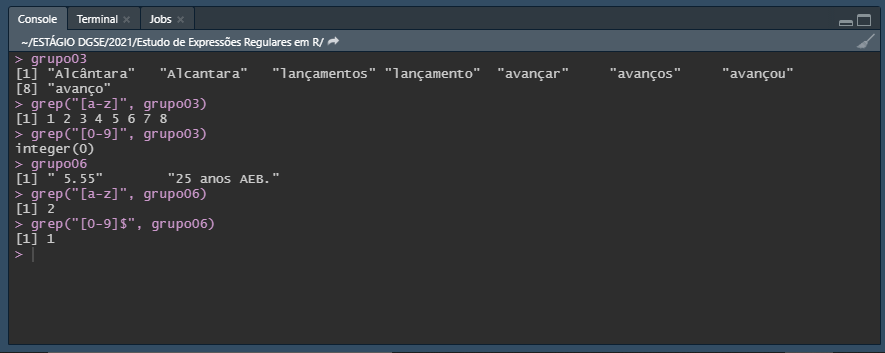
\includegraphics[width=0.7\linewidth]{style/image/caso09.png}
    \caption{Agrupamento}
    \label{fig:grep01}
\end{figure}
\subsection{Ponto}
O ponto, $.$ serve para isolar qualquer termo. Nesse caso foi feito exemplo realizando uma combinação de expressões regulares a fim de demonstrar a sua funcionalidade.
\begin{figure}[htb!]
    \centering
    \includegraphics[width=0.7\linewidth]{style/image/caso07.png}
    \caption{Ponto}
    \label{fig:Ponto}
\end{figure}
\subsection{Agrupamento}
É possível realizar o agrupamento dos padrões que devem ser encontrados no grupo de texto que está sendo tratado e para isso as expressões regulares se tornam utéis. Dessa forma é possível escolher quais palavras padrões você quer visualizar. Esse agrupamento pode ser feito a partir da função grep().
\begin{figure}[htb!]
    \centering
    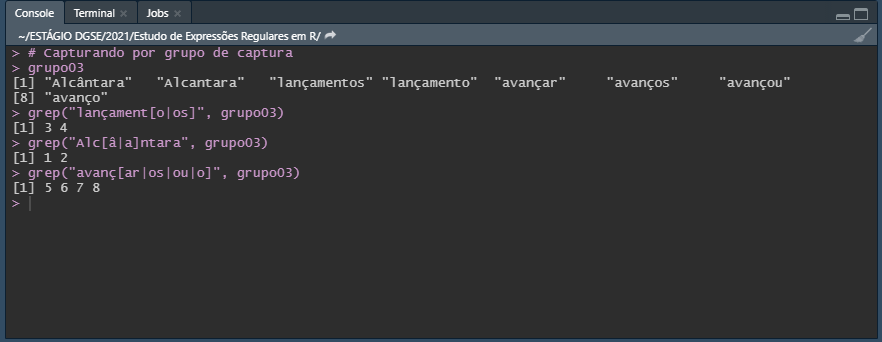
\includegraphics[width=0.7\linewidth]{style/image/caso10.png}
    \caption{Agrupamento}
    \label{fig:grep}
\end{figure}
Na opção de agrupamento ele sinaliza pelo índice aonde se encontra o padrão procurado, para obter a visualização desse padrão tem-se a opção de $value = True$ adicionada ao script, dessa forma os valores que correspondentes serão apresentados.
\begin{figure}[htb!]
    \centering
    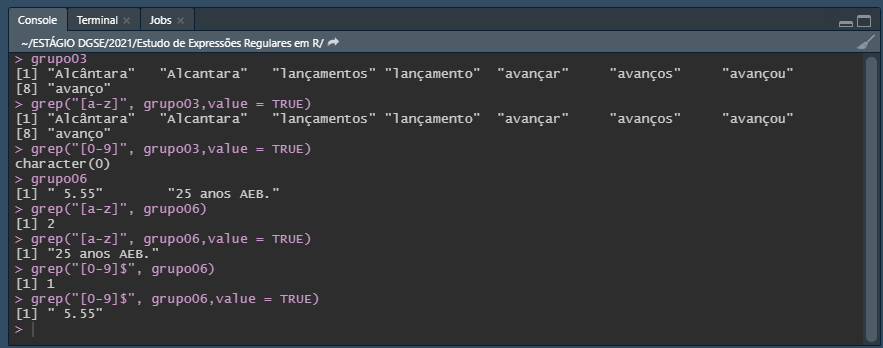
\includegraphics[width=0.7\linewidth]{style/image/caso11.png}
    \caption{Agrupamento com value}
    \label{fig:grepwithvalue}
\end{figure}
\section{Script de teste}
O script realiza a busca por termos como alcântara e alcantara e um segundo teste foi adicionado utilizando a busca por base de alcântara. Essa ecolha foi feita pois aparecem menos outliers possibilitando identificar mais rápido se o dado foi tratado ou não.
Foi adicionado ao script busca alcântara o pacote tidyverse e posteriormente no momento de realizar a busca com a função search tweets foi mantida a busca por Alcântara. Tendo essa busca é feito um tratamento de forma que sejam realizas as extrações apenas dos padrões que são necessários para o estudo.
Foi utilizado inicialmente um filtro que utiliza apenas as colunas desejadas para análise, esse método foi adicionado pois ele coleta apenas as colunas de interesse para o banco de dados do aebsocialdata.
No teste , foi notado que ao realizar a busca utilizando o str detect é possível identificar com true ou false se o elemento que foi colocado para busca foi encontrado ou não.Mas também foi notado que ele não permite que seja exibido a tabela com os valores utilizando apenas essa forma do str detect.As imagens adicionadas abaixo são relacionadas a busca por base de alcântara no twitter utilizando a função search tweets.
\begin{figure}[htb!]
    \centering
    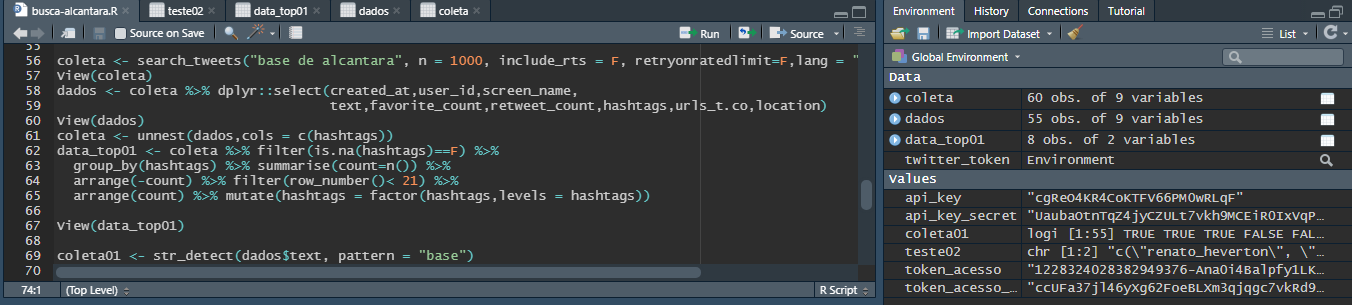
\includegraphics[width=0.9\linewidth]{style/image/teste03.png}
    \caption{script}
    \label{fig:script}
\end{figure}

É possível ver que é realizada a redução de colunas no momento da coleta, sendo essa adaptação útil para o script de coleta atual.

\begin{figure}[htb!]
    \centering
    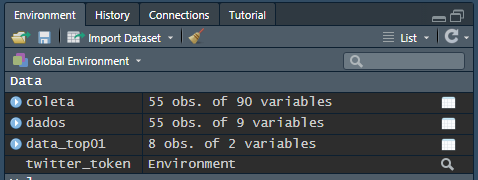
\includegraphics[width=0.5\linewidth]{style/image/teste05.png}
    \caption{Tratamento das colunas}
    \label{fig:coluna}
\end{figure}

\begin{figure}[htb!]
    \centering
    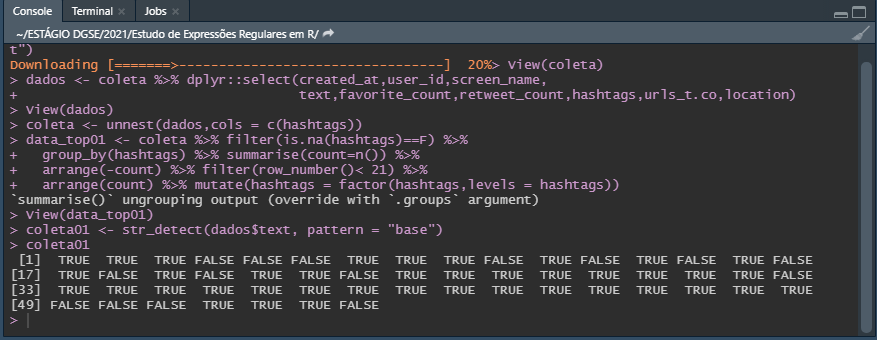
\includegraphics[width=0.9\linewidth]{style/image/teste02.png}
    \caption{str detect}
    \label{fig:str_detect}
\end{figure}
Foi feito um ranking das hashtags que foram citadas na coleta direto no script. 
\begin{figure}[htb!]
    \centering
    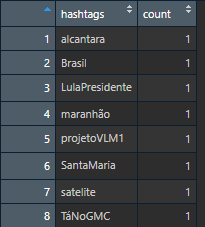
\includegraphics[width=0.5\linewidth]{style/image/teste04-hashtags.png}
    \caption{hashtags}
    \label{fig:hashtags}
\end{figure}

\section{Conclusão}
Diante do que foi apresentado, verifica-se a possibilidade de inserir algumas expressões regulares no script de coleta do projeto sobre o PDI-CEA. Visando na detecção de expressões que são de interesse do projeto e manter apenas ela no script ou da retirada de outliers.
As expressões seriam utilizadas de maneira preferencial no momento da coleta e ao invés de ser salvo o conjunto de textos e realizar o tratamento depois, no momento da coleta realizar esse tratamento com expressões regulares e salvar o arquivo já tratado no script principal.
São necessárias adaptações no script para que ele funcione de maneira ideal para o projeto. 
\bigskip
\end{document}
